\documentclass[tikz, border=10pt]{standalone}
\usepackage{tikz}
\usepackage{amsmath}
\usetikzlibrary{positioning, arrows.meta, shapes, backgrounds, fit, calc}

\usepackage{helvet}
\renewcommand{\familydefault}{\sfdefault}
\usepackage{sansmath}
\sansmath

% UCL brand accessible data-viz palette (matches marvel_algorithm.tex)
\definecolor{uclDarkPurple}{HTML}{361A54}
\definecolor{uclLightPink}{HTML}{E645AB}
\definecolor{uclLightOrange}{HTML}{E66C37}
\definecolor{uclLightGreen}{HTML}{1AAB40}
\definecolor{uclLightBlue}{HTML}{118DFF}
\definecolor{uclDarkRed}{HTML}{751441}

% Layer control: 1 = clean network, 2 = +orphan cluster, 3 = +mislabeled edge,
% 4 = +partial new-source path that almost, but doesn't quite, close the loop.
% Default (plain compile) shows the full, combined state.
% Per-layer builds: pdflatex -jobname=marvel_breaks_N "\def\layer{N}\documentclass[tikz, border=10pt]{standalone}
\usepackage{tikz}
\usepackage{amsmath}
\usetikzlibrary{positioning, arrows.meta, shapes, backgrounds, fit, calc}

\usepackage{helvet}
\renewcommand{\familydefault}{\sfdefault}
\usepackage{sansmath}
\sansmath

% UCL brand accessible data-viz palette (matches marvel_algorithm.tex)
\definecolor{uclDarkPurple}{HTML}{361A54}
\definecolor{uclLightPink}{HTML}{E645AB}
\definecolor{uclLightOrange}{HTML}{E66C37}
\definecolor{uclLightGreen}{HTML}{1AAB40}
\definecolor{uclLightBlue}{HTML}{118DFF}
\definecolor{uclDarkRed}{HTML}{751441}

% Layer control: 1 = clean network, 2 = +orphan cluster, 3 = +mislabeled edge,
% 4 = +partial new-source path that almost, but doesn't quite, close the loop.
% Default (plain compile) shows the full, combined state.
% Per-layer builds: pdflatex -jobname=marvel_breaks_N "\def\layer{N}\documentclass[tikz, border=10pt]{standalone}
\usepackage{tikz}
\usepackage{amsmath}
\usetikzlibrary{positioning, arrows.meta, shapes, backgrounds, fit, calc}

\usepackage{helvet}
\renewcommand{\familydefault}{\sfdefault}
\usepackage{sansmath}
\sansmath

% UCL brand accessible data-viz palette (matches marvel_algorithm.tex)
\definecolor{uclDarkPurple}{HTML}{361A54}
\definecolor{uclLightPink}{HTML}{E645AB}
\definecolor{uclLightOrange}{HTML}{E66C37}
\definecolor{uclLightGreen}{HTML}{1AAB40}
\definecolor{uclLightBlue}{HTML}{118DFF}
\definecolor{uclDarkRed}{HTML}{751441}

% Layer control: 1 = clean network, 2 = +orphan cluster, 3 = +mislabeled edge,
% 4 = +partial new-source path that almost, but doesn't quite, close the loop.
% Default (plain compile) shows the full, combined state.
% Per-layer builds: pdflatex -jobname=marvel_breaks_N "\def\layer{N}\documentclass[tikz, border=10pt]{standalone}
\usepackage{tikz}
\usepackage{amsmath}
\usetikzlibrary{positioning, arrows.meta, shapes, backgrounds, fit, calc}

\usepackage{helvet}
\renewcommand{\familydefault}{\sfdefault}
\usepackage{sansmath}
\sansmath

% UCL brand accessible data-viz palette (matches marvel_algorithm.tex)
\definecolor{uclDarkPurple}{HTML}{361A54}
\definecolor{uclLightPink}{HTML}{E645AB}
\definecolor{uclLightOrange}{HTML}{E66C37}
\definecolor{uclLightGreen}{HTML}{1AAB40}
\definecolor{uclLightBlue}{HTML}{118DFF}
\definecolor{uclDarkRed}{HTML}{751441}

% Layer control: 1 = clean network, 2 = +orphan cluster, 3 = +mislabeled edge,
% 4 = +partial new-source path that almost, but doesn't quite, close the loop.
% Default (plain compile) shows the full, combined state.
% Per-layer builds: pdflatex -jobname=marvel_breaks_N "\def\layer{N}\input{marvel_breaks.tex}"
\providecommand{\layer}{4}

\begin{document}

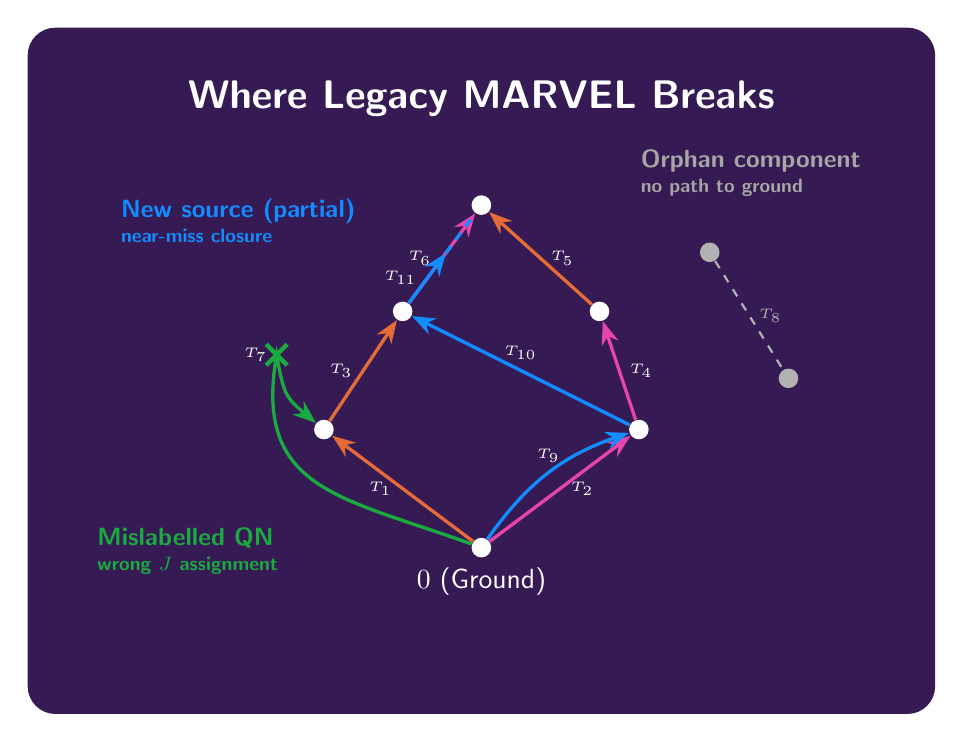
\begin{tikzpicture}[
    font=\sffamily,
    >=Stealth,
    node distance=1cm,
    every node/.style={text=white},
    level_dot/.style={circle, fill=white, inner sep=2.5pt},
    orphan_dot/.style={circle, fill=gray!60, inner sep=2.5pt},
    srcA/.style={->, very thick, color=uclLightOrange},
    srcB/.style={->, very thick, color=uclLightPink},
    srcC/.style={->, very thick, color=uclLightBlue},
    srcC_gap/.style={-, very thick, dashed, color=uclLightBlue},
    orphan_edge/.style={-, thick, dashed, gray!60},
    flagged_edge/.style={->, very thick, color=uclLightGreen},
    flag_mark/.style={cross out, draw=uclLightGreen, ultra thick, minimum size=6pt, inner sep=0pt},
    panel_bg/.style={rounded corners=10pt, inner sep=16pt, draw=none},
    heading/.style={font=\bfseries\Large, align=center, anchor=south},
    caption_style/.style={font=\bfseries\small, align=left, anchor=west, text=gray!70!white}
]

\begin{scope}[local bounding box=net]
    % Fixed-extent invisible strut: keeps the canvas identical across all 3
    % layer compiles (standalone auto-crops to content, which would otherwise
    % shift per-layer since layers 2/3 add content further out) so the 3
    % exported PNGs stack pixel-for-pixel in the slide deck.
    \path (-0.8,-2.3) rectangle (9.6, 5.1);

    % Heading
    \node[heading] at (4.4, 4.6) {Where Legacy MARVEL Breaks};

    % --- MAIN NETWORK (6 nodes), centred on the fixed canvas ---
    \node[level_dot, label={[text=white]below:{$0$ (Ground)}}] (G) at (4.4, -0.75) {};
    \node[level_dot] (A) at (2.4, 0.75) {};
    \node[level_dot] (B) at (6.4, 0.75) {};
    \node[level_dot] (C) at (3.4, 2.25) {};
    \node[level_dot] (D) at (5.9, 2.25) {};
    \node[level_dot] (E) at (4.4, 3.6) {};

    \draw[srcA] (G) -- (A) node[midway, left, font=\tiny] {$T_1$};
    \draw[srcB] (G) -- (B) node[midway, right, font=\tiny] {$T_2$};
    \draw[srcA] (A) -- (C) node[midway, left, font=\tiny] {$T_3$};
    \draw[srcB] (B) -- (D) node[midway, right, font=\tiny] {$T_4$};
    \draw[srcA] (D) -- (E) node[midway, right, font=\tiny] {$T_5$};
    \draw[srcB] (C) -- (E) node[midway, left, font=\tiny] {$T_6$};

    % --- LAYER 2: orphan sub-cluster (disconnected, greyed, dashed) ---
    \ifnum\layer>1
        \node[orphan_dot] (X) at (7.3, 3.0) {};
        \node[orphan_dot] (Y) at (8.3, 1.4) {};
        \draw[orphan_edge] (X) -- (Y) node[midway, right, font=\tiny, text=gray!60] {$T_8$};
        \node[caption_style, align=left] at (6.3, 4.0) {Orphan component\\[-2pt]{\scriptsize no path to ground}};
    \fi

    % --- LAYER 3: mislabeled transition, ground -> T1's terminus (A) ---
    % Curves out, curls back on the left, and does a 180 right above A before
    % dropping in -- shows its path is absurdly roundabout for how close G
    % and A actually are (T1 gets there directly, right alongside it).
    \ifnum\layer>2
        \coordinate (t7curl) at ($(A)+(-0.6,0.95)$);
        \draw[flagged_edge] (G) to[out=160, in=260, looseness=1.3] (t7curl)
            to[out=-80, in=140, looseness=1.3] (A);
        \node[left, font=\tiny, text=white] at (t7curl) {$T_7$};
        \node[flag_mark] at (t7curl) {};
        \node[caption_style, align=left, text=uclLightGreen] at (-0.6, -0.8) {Mislabelled QN\\[-2pt]{\scriptsize wrong $J$ assignment}};
    \fi

    % --- LAYER 4: new source, partial path that almost closes the loop ---
    % Traces G -> B (parallel to T2), B -> C (new link, "top of T3"), then
    % follows T6's direction from C but stops short of E -- the missing last
    % transition is shown as a dashed gap, since it was never measured.
    \ifnum\layer>3
        \draw[srcC] (G) to[bend left=18] node[midway, above, font=\tiny] {$T_9$} (B);
        \draw[srcC] (B) -- (C) node[midway, above, font=\tiny] {$T_{10}$};
        \draw[srcC] (C) -- ($(C)!0.55!(E)$) node[midway, left, font=\tiny] {$T_{11}$};
        \draw[srcC_gap] ($(C)!0.55!(E)$) -- ($(C)!0.9!(E)$);
        \node[caption_style, align=left, text=uclLightBlue] at (-0.3, 3.4) {New source (partial)\\[-2pt]{\scriptsize near-miss closure}};
    \fi
\end{scope}

\begin{scope}[on background layer]
    \node[panel_bg, fill=uclDarkPurple, fit=(net)] {};
\end{scope}

\path[use as bounding box] (net.south west) rectangle (net.north east);

\end{tikzpicture}
\end{document}
"
\providecommand{\layer}{4}

\begin{document}

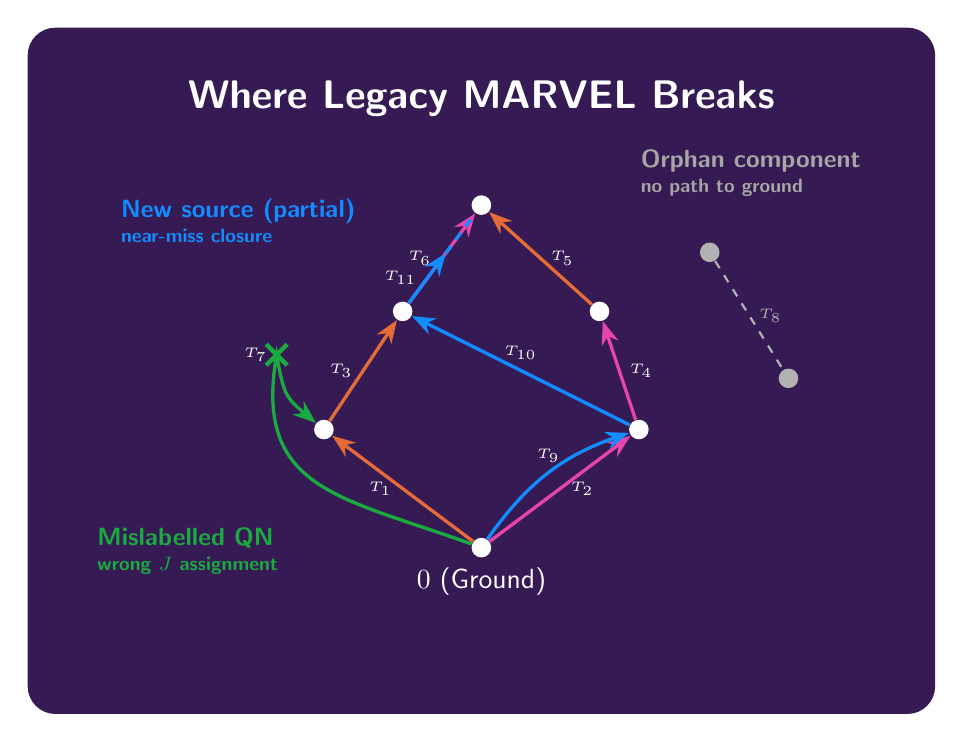
\begin{tikzpicture}[
    font=\sffamily,
    >=Stealth,
    node distance=1cm,
    every node/.style={text=white},
    level_dot/.style={circle, fill=white, inner sep=2.5pt},
    orphan_dot/.style={circle, fill=gray!60, inner sep=2.5pt},
    srcA/.style={->, very thick, color=uclLightOrange},
    srcB/.style={->, very thick, color=uclLightPink},
    srcC/.style={->, very thick, color=uclLightBlue},
    srcC_gap/.style={-, very thick, dashed, color=uclLightBlue},
    orphan_edge/.style={-, thick, dashed, gray!60},
    flagged_edge/.style={->, very thick, color=uclLightGreen},
    flag_mark/.style={cross out, draw=uclLightGreen, ultra thick, minimum size=6pt, inner sep=0pt},
    panel_bg/.style={rounded corners=10pt, inner sep=16pt, draw=none},
    heading/.style={font=\bfseries\Large, align=center, anchor=south},
    caption_style/.style={font=\bfseries\small, align=left, anchor=west, text=gray!70!white}
]

\begin{scope}[local bounding box=net]
    % Fixed-extent invisible strut: keeps the canvas identical across all 3
    % layer compiles (standalone auto-crops to content, which would otherwise
    % shift per-layer since layers 2/3 add content further out) so the 3
    % exported PNGs stack pixel-for-pixel in the slide deck.
    \path (-0.8,-2.3) rectangle (9.6, 5.1);

    % Heading
    \node[heading] at (4.4, 4.6) {Where Legacy MARVEL Breaks};

    % --- MAIN NETWORK (6 nodes), centred on the fixed canvas ---
    \node[level_dot, label={[text=white]below:{$0$ (Ground)}}] (G) at (4.4, -0.75) {};
    \node[level_dot] (A) at (2.4, 0.75) {};
    \node[level_dot] (B) at (6.4, 0.75) {};
    \node[level_dot] (C) at (3.4, 2.25) {};
    \node[level_dot] (D) at (5.9, 2.25) {};
    \node[level_dot] (E) at (4.4, 3.6) {};

    \draw[srcA] (G) -- (A) node[midway, left, font=\tiny] {$T_1$};
    \draw[srcB] (G) -- (B) node[midway, right, font=\tiny] {$T_2$};
    \draw[srcA] (A) -- (C) node[midway, left, font=\tiny] {$T_3$};
    \draw[srcB] (B) -- (D) node[midway, right, font=\tiny] {$T_4$};
    \draw[srcA] (D) -- (E) node[midway, right, font=\tiny] {$T_5$};
    \draw[srcB] (C) -- (E) node[midway, left, font=\tiny] {$T_6$};

    % --- LAYER 2: orphan sub-cluster (disconnected, greyed, dashed) ---
    \ifnum\layer>1
        \node[orphan_dot] (X) at (7.3, 3.0) {};
        \node[orphan_dot] (Y) at (8.3, 1.4) {};
        \draw[orphan_edge] (X) -- (Y) node[midway, right, font=\tiny, text=gray!60] {$T_8$};
        \node[caption_style, align=left] at (6.3, 4.0) {Orphan component\\[-2pt]{\scriptsize no path to ground}};
    \fi

    % --- LAYER 3: mislabeled transition, ground -> T1's terminus (A) ---
    % Curves out, curls back on the left, and does a 180 right above A before
    % dropping in -- shows its path is absurdly roundabout for how close G
    % and A actually are (T1 gets there directly, right alongside it).
    \ifnum\layer>2
        \coordinate (t7curl) at ($(A)+(-0.6,0.95)$);
        \draw[flagged_edge] (G) to[out=160, in=260, looseness=1.3] (t7curl)
            to[out=-80, in=140, looseness=1.3] (A);
        \node[left, font=\tiny, text=white] at (t7curl) {$T_7$};
        \node[flag_mark] at (t7curl) {};
        \node[caption_style, align=left, text=uclLightGreen] at (-0.6, -0.8) {Mislabelled QN\\[-2pt]{\scriptsize wrong $J$ assignment}};
    \fi

    % --- LAYER 4: new source, partial path that almost closes the loop ---
    % Traces G -> B (parallel to T2), B -> C (new link, "top of T3"), then
    % follows T6's direction from C but stops short of E -- the missing last
    % transition is shown as a dashed gap, since it was never measured.
    \ifnum\layer>3
        \draw[srcC] (G) to[bend left=18] node[midway, above, font=\tiny] {$T_9$} (B);
        \draw[srcC] (B) -- (C) node[midway, above, font=\tiny] {$T_{10}$};
        \draw[srcC] (C) -- ($(C)!0.55!(E)$) node[midway, left, font=\tiny] {$T_{11}$};
        \draw[srcC_gap] ($(C)!0.55!(E)$) -- ($(C)!0.9!(E)$);
        \node[caption_style, align=left, text=uclLightBlue] at (-0.3, 3.4) {New source (partial)\\[-2pt]{\scriptsize near-miss closure}};
    \fi
\end{scope}

\begin{scope}[on background layer]
    \node[panel_bg, fill=uclDarkPurple, fit=(net)] {};
\end{scope}

\path[use as bounding box] (net.south west) rectangle (net.north east);

\end{tikzpicture}
\end{document}
"
\providecommand{\layer}{4}

\begin{document}

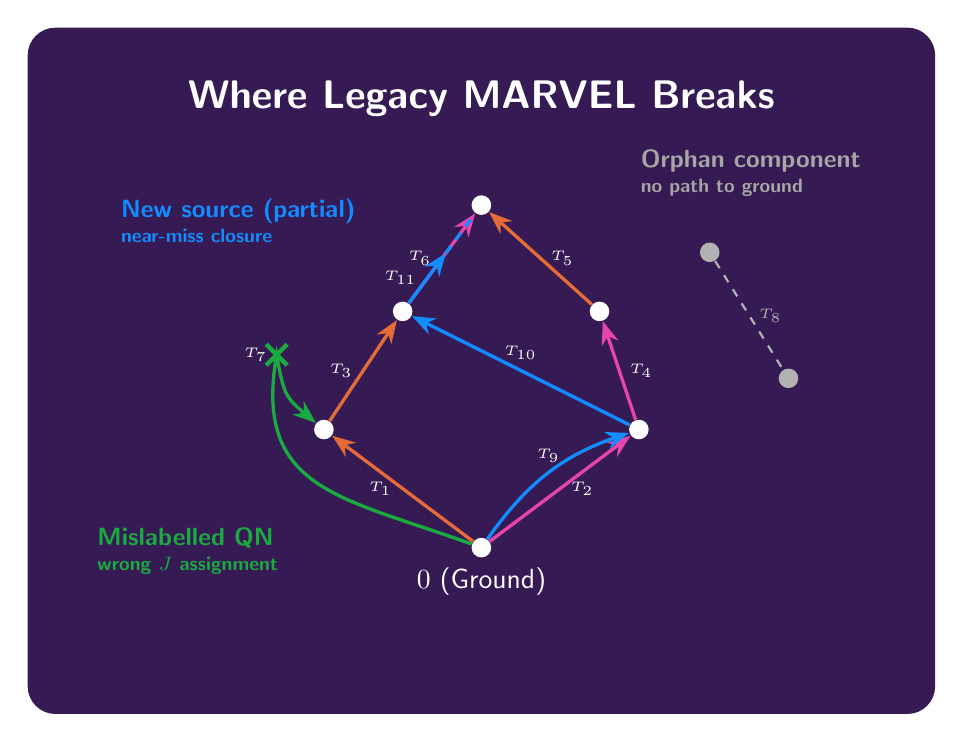
\begin{tikzpicture}[
    font=\sffamily,
    >=Stealth,
    node distance=1cm,
    every node/.style={text=white},
    level_dot/.style={circle, fill=white, inner sep=2.5pt},
    orphan_dot/.style={circle, fill=gray!60, inner sep=2.5pt},
    srcA/.style={->, very thick, color=uclLightOrange},
    srcB/.style={->, very thick, color=uclLightPink},
    srcC/.style={->, very thick, color=uclLightBlue},
    srcC_gap/.style={-, very thick, dashed, color=uclLightBlue},
    orphan_edge/.style={-, thick, dashed, gray!60},
    flagged_edge/.style={->, very thick, color=uclLightGreen},
    flag_mark/.style={cross out, draw=uclLightGreen, ultra thick, minimum size=6pt, inner sep=0pt},
    panel_bg/.style={rounded corners=10pt, inner sep=16pt, draw=none},
    heading/.style={font=\bfseries\Large, align=center, anchor=south},
    caption_style/.style={font=\bfseries\small, align=left, anchor=west, text=gray!70!white}
]

\begin{scope}[local bounding box=net]
    % Fixed-extent invisible strut: keeps the canvas identical across all 3
    % layer compiles (standalone auto-crops to content, which would otherwise
    % shift per-layer since layers 2/3 add content further out) so the 3
    % exported PNGs stack pixel-for-pixel in the slide deck.
    \path (-0.8,-2.3) rectangle (9.6, 5.1);

    % Heading
    \node[heading] at (4.4, 4.6) {Where Legacy MARVEL Breaks};

    % --- MAIN NETWORK (6 nodes), centred on the fixed canvas ---
    \node[level_dot, label={[text=white]below:{$0$ (Ground)}}] (G) at (4.4, -0.75) {};
    \node[level_dot] (A) at (2.4, 0.75) {};
    \node[level_dot] (B) at (6.4, 0.75) {};
    \node[level_dot] (C) at (3.4, 2.25) {};
    \node[level_dot] (D) at (5.9, 2.25) {};
    \node[level_dot] (E) at (4.4, 3.6) {};

    \draw[srcA] (G) -- (A) node[midway, left, font=\tiny] {$T_1$};
    \draw[srcB] (G) -- (B) node[midway, right, font=\tiny] {$T_2$};
    \draw[srcA] (A) -- (C) node[midway, left, font=\tiny] {$T_3$};
    \draw[srcB] (B) -- (D) node[midway, right, font=\tiny] {$T_4$};
    \draw[srcA] (D) -- (E) node[midway, right, font=\tiny] {$T_5$};
    \draw[srcB] (C) -- (E) node[midway, left, font=\tiny] {$T_6$};

    % --- LAYER 2: orphan sub-cluster (disconnected, greyed, dashed) ---
    \ifnum\layer>1
        \node[orphan_dot] (X) at (7.3, 3.0) {};
        \node[orphan_dot] (Y) at (8.3, 1.4) {};
        \draw[orphan_edge] (X) -- (Y) node[midway, right, font=\tiny, text=gray!60] {$T_8$};
        \node[caption_style, align=left] at (6.3, 4.0) {Orphan component\\[-2pt]{\scriptsize no path to ground}};
    \fi

    % --- LAYER 3: mislabeled transition, ground -> T1's terminus (A) ---
    % Curves out, curls back on the left, and does a 180 right above A before
    % dropping in -- shows its path is absurdly roundabout for how close G
    % and A actually are (T1 gets there directly, right alongside it).
    \ifnum\layer>2
        \coordinate (t7curl) at ($(A)+(-0.6,0.95)$);
        \draw[flagged_edge] (G) to[out=160, in=260, looseness=1.3] (t7curl)
            to[out=-80, in=140, looseness=1.3] (A);
        \node[left, font=\tiny, text=white] at (t7curl) {$T_7$};
        \node[flag_mark] at (t7curl) {};
        \node[caption_style, align=left, text=uclLightGreen] at (-0.6, -0.8) {Mislabelled QN\\[-2pt]{\scriptsize wrong $J$ assignment}};
    \fi

    % --- LAYER 4: new source, partial path that almost closes the loop ---
    % Traces G -> B (parallel to T2), B -> C (new link, "top of T3"), then
    % follows T6's direction from C but stops short of E -- the missing last
    % transition is shown as a dashed gap, since it was never measured.
    \ifnum\layer>3
        \draw[srcC] (G) to[bend left=18] node[midway, above, font=\tiny] {$T_9$} (B);
        \draw[srcC] (B) -- (C) node[midway, above, font=\tiny] {$T_{10}$};
        \draw[srcC] (C) -- ($(C)!0.55!(E)$) node[midway, left, font=\tiny] {$T_{11}$};
        \draw[srcC_gap] ($(C)!0.55!(E)$) -- ($(C)!0.9!(E)$);
        \node[caption_style, align=left, text=uclLightBlue] at (-0.3, 3.4) {New source (partial)\\[-2pt]{\scriptsize near-miss closure}};
    \fi
\end{scope}

\begin{scope}[on background layer]
    \node[panel_bg, fill=uclDarkPurple, fit=(net)] {};
\end{scope}

\path[use as bounding box] (net.south west) rectangle (net.north east);

\end{tikzpicture}
\end{document}
"
\providecommand{\layer}{4}

\begin{document}

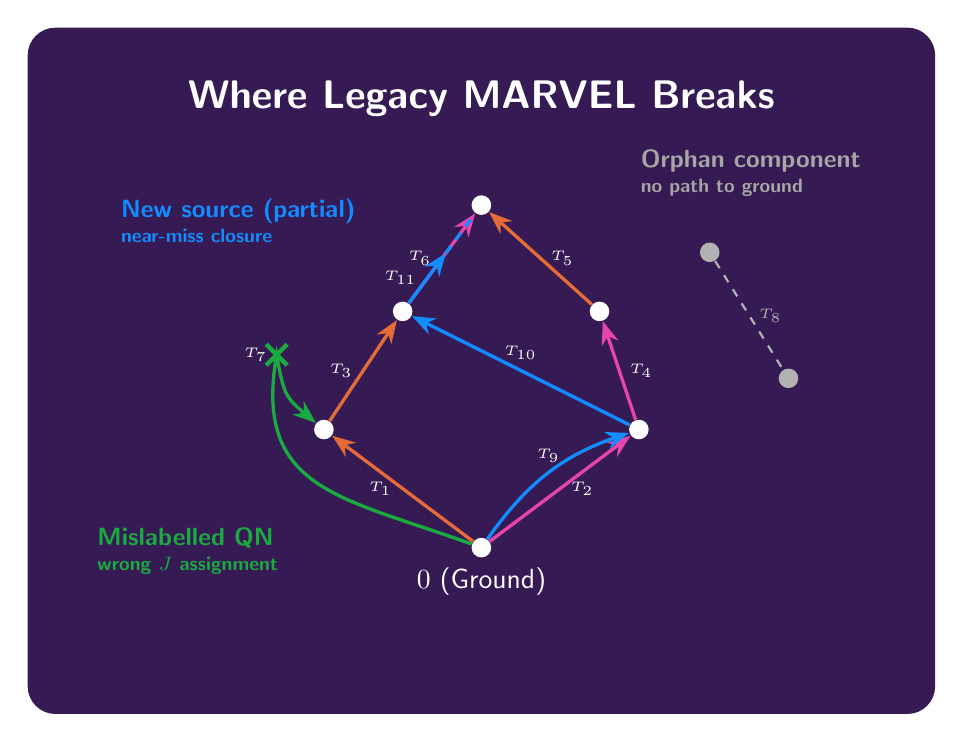
\begin{tikzpicture}[
    font=\sffamily,
    >=Stealth,
    node distance=1cm,
    every node/.style={text=white},
    level_dot/.style={circle, fill=white, inner sep=2.5pt},
    orphan_dot/.style={circle, fill=gray!60, inner sep=2.5pt},
    srcA/.style={->, very thick, color=uclLightOrange},
    srcB/.style={->, very thick, color=uclLightPink},
    srcC/.style={->, very thick, color=uclLightBlue},
    srcC_gap/.style={-, very thick, dashed, color=uclLightBlue},
    orphan_edge/.style={-, thick, dashed, gray!60},
    flagged_edge/.style={->, very thick, color=uclLightGreen},
    flag_mark/.style={cross out, draw=uclLightGreen, ultra thick, minimum size=6pt, inner sep=0pt},
    panel_bg/.style={rounded corners=10pt, inner sep=16pt, draw=none},
    heading/.style={font=\bfseries\Large, align=center, anchor=south},
    caption_style/.style={font=\bfseries\small, align=left, anchor=west, text=gray!70!white}
]

\begin{scope}[local bounding box=net]
    % Fixed-extent invisible strut: keeps the canvas identical across all 3
    % layer compiles (standalone auto-crops to content, which would otherwise
    % shift per-layer since layers 2/3 add content further out) so the 3
    % exported PNGs stack pixel-for-pixel in the slide deck.
    \path (-0.8,-2.3) rectangle (9.6, 5.1);

    % Heading
    \node[heading] at (4.4, 4.6) {Where Legacy MARVEL Breaks};

    % --- MAIN NETWORK (6 nodes), centred on the fixed canvas ---
    \node[level_dot, label={[text=white]below:{$0$ (Ground)}}] (G) at (4.4, -0.75) {};
    \node[level_dot] (A) at (2.4, 0.75) {};
    \node[level_dot] (B) at (6.4, 0.75) {};
    \node[level_dot] (C) at (3.4, 2.25) {};
    \node[level_dot] (D) at (5.9, 2.25) {};
    \node[level_dot] (E) at (4.4, 3.6) {};

    \draw[srcA] (G) -- (A) node[midway, left, font=\tiny] {$T_1$};
    \draw[srcB] (G) -- (B) node[midway, right, font=\tiny] {$T_2$};
    \draw[srcA] (A) -- (C) node[midway, left, font=\tiny] {$T_3$};
    \draw[srcB] (B) -- (D) node[midway, right, font=\tiny] {$T_4$};
    \draw[srcA] (D) -- (E) node[midway, right, font=\tiny] {$T_5$};
    \draw[srcB] (C) -- (E) node[midway, left, font=\tiny] {$T_6$};

    % --- LAYER 2: orphan sub-cluster (disconnected, greyed, dashed) ---
    \ifnum\layer>1
        \node[orphan_dot] (X) at (7.3, 3.0) {};
        \node[orphan_dot] (Y) at (8.3, 1.4) {};
        \draw[orphan_edge] (X) -- (Y) node[midway, right, font=\tiny, text=gray!60] {$T_8$};
        \node[caption_style, align=left] at (6.3, 4.0) {Orphan component\\[-2pt]{\scriptsize no path to ground}};
    \fi

    % --- LAYER 3: mislabeled transition, ground -> T1's terminus (A) ---
    % Curves out, curls back on the left, and does a 180 right above A before
    % dropping in -- shows its path is absurdly roundabout for how close G
    % and A actually are (T1 gets there directly, right alongside it).
    \ifnum\layer>2
        \coordinate (t7curl) at ($(A)+(-0.6,0.95)$);
        \draw[flagged_edge] (G) to[out=160, in=260, looseness=1.3] (t7curl)
            to[out=-80, in=140, looseness=1.3] (A);
        \node[left, font=\tiny, text=white] at (t7curl) {$T_7$};
        \node[flag_mark] at (t7curl) {};
        \node[caption_style, align=left, text=uclLightGreen] at (-0.6, -0.8) {Mislabelled QN\\[-2pt]{\scriptsize wrong $J$ assignment}};
    \fi

    % --- LAYER 4: new source, partial path that almost closes the loop ---
    % Traces G -> B (parallel to T2), B -> C (new link, "top of T3"), then
    % follows T6's direction from C but stops short of E -- the missing last
    % transition is shown as a dashed gap, since it was never measured.
    \ifnum\layer>3
        \draw[srcC] (G) to[bend left=18] node[midway, above, font=\tiny] {$T_9$} (B);
        \draw[srcC] (B) -- (C) node[midway, above, font=\tiny] {$T_{10}$};
        \draw[srcC] (C) -- ($(C)!0.55!(E)$) node[midway, left, font=\tiny] {$T_{11}$};
        \draw[srcC_gap] ($(C)!0.55!(E)$) -- ($(C)!0.9!(E)$);
        \node[caption_style, align=left, text=uclLightBlue] at (-0.3, 3.4) {New source (partial)\\[-2pt]{\scriptsize near-miss closure}};
    \fi
\end{scope}

\begin{scope}[on background layer]
    \node[panel_bg, fill=uclDarkPurple, fit=(net)] {};
\end{scope}

\path[use as bounding box] (net.south west) rectangle (net.north east);

\end{tikzpicture}
\end{document}
